\documentclass[11pt,letterpaper]{article}
\usepackage[T1]{fontenc}
\usepackage{lmodern,microtype}
\usepackage[margin=1in,headheight=15pt]{geometry}
\usepackage{amsmath,amssymb,amsthm,mathtools}
\usepackage{booktabs,tabularx,longtable,array}
\usepackage{graphicx,xcolor,enumitem}
\usepackage{fancyhdr}
\usepackage[colorlinks=true,linkcolor=teal!65!black,citecolor=teal!65!black,urlcolor=teal!65!black]{hyperref}
\usepackage[font=small,labelfont=bf]{caption}
\hypersetup{pdftitle={Exact p-adic symplectic corner laws},pdfauthor={Research note prepared for Vladimir Reshetnikov},pdfsubject={Exact local matrix distributions, total variation, and cokernels}}
\newtheorem{theorem}{Theorem}[section]
\newtheorem{lemma}[theorem]{Lemma}
\newtheorem{corollary}[theorem]{Corollary}
\newtheorem{proposition}[theorem]{Proposition}
\theoremstyle{remark}
\newtheorem{remark}[theorem]{Remark}
\newtheorem{example}[theorem]{Example}
\newcommand{\OO}{\mathcal O}
\newcommand{\TV}{\operatorname{TV}}
\newcommand{\Sp}{\operatorname{Sp}}
\newcommand{\Mat}{\operatorname{Mat}}
\newcommand{\coker}{\operatorname{coker}}
\newcommand{\artifact}[1]{\texttt{\detokenize{#1}}}
\setlist{itemsep=3pt,topsep=5pt}
\setlength{\emergencystretch}{2em}
\pagestyle{fancy}
\fancyhf{}
\fancyhead[L]{\small Exact symplectic corner laws}
\fancyhead[R]{\small Research note}
\fancyfoot[C]{\thepage}
\title{\textbf{Exact $p$-adic symplectic corner laws}\\[5pt]
\large One residue digit attains the full distinguishing distance}
\author{Prepared for Vladimir Reshetnikov}
\date{26 November 2026}
\begin{document}
\maketitle
\begin{abstract}
We extend finite-field symplectic compression methods appearing in the
\texttt{grh-lean} research program and the associated \texttt{ProveIt} article
to all congruence precisions over an arbitrary complete discrete valuation
ring with finite residue field. For a Haar symplectic transformation in
dimension $2g\ge4$, compressed between two symplectic planes, we derive its
exact matrix density in terms of $v(1-\det A)$. Its total variation distance
from four independent uniform entries is
\[
 \left(1-q^{-1}+q^{-3}\right)\frac{q^2-1}{q^{2g}-1}
\]
at every finite precision and over the complete ring. A determinant test
modulo the residue field is already optimal, even though higher digits
change the likelihood ratio. We determine exactly the bias discarded by
uniformly completing any finite precision, and prove that all nontrivial
cokernel types have the same correction factor relative to the independent
model. An exact rejection sampler needs $8/5$ proposals on average.
For arbitrary primitive rectangular frames, the differential defect is
exactly $\binom{s}{2}$, where $s$ is their reduced intersection dimension;
this gives an explicit precision-uniform $O(q^{-4g})$ lifting error at
fixed frame dimensions. The proofs include residue characteristic two
and do not assume RH or GRH. Exact finite-ring computations accompany
the proofs. The novelty claim is limited to the statements derived here
and the primary literature examined, not an assertion of exhaustive priority.
\end{abstract}
\setcounter{tocdepth}{1}
\tableofcontents
\newpage
\section{Source analysis and the advance developed here}
\label{sec:context}

\subsection{What was inspected}

The starting points are the readable edition of \texttt{lsernau/grh-lean}
and the \texttt{ProveIt} merged article \cite{Sernau2026,ProveIt2026},
at the following respective commits:
\begin{center}\small
\texttt{72fead102f663d5c7a407964a13dc0cf9d977207}\\
\texttt{fc9889c80312959aee9893ab21bfc9e741719e88}.
\end{center}
Source identities are pinned so that
later repository changes cannot silently alter the comparison.

The upstream exported statements concern the Riemann hypothesis and
GRH for Dirichlet $L$-functions over $\mathbb Q$, including imprimitive
characters in the open critical strip. They do not quantify over
general Artin or automorphic $L$-functions. The repository reports
machine checks and dependency on the usual three Lean axioms
\texttt{propext}, \texttt{Classical.choice} and \texttt{Quot.sound}.
The present investigation inspected the statements, entry point,
reading guide, prime-error reduction, one-sided criterion, and related
source files. It did not rebuild the full upstream development or
repeat an independent kernel replay. These are statements about the
scope and reported status of that source, not a new verification of it.

At the pinned commit, the article's README describes a 621-page merger
of 103 reports, counting 760 theorem-like results. It explicitly says
that it is a compilation, that the input Dirichlet-GRH theorem is taken
as given, and that the merged mathematical claims were not independently
recomputed or formalized in that compilation. All 21 section source
files and the bibliography were retrieved for comparison. The source
analysis below uses the article as a record of the existing methods and
results; the new arguments in this note are supplied in full.

\subsection{Which mechanism transfers}

Three mechanisms organize the source proof and its existing extensions.
First, nonnegative prime-power weights and a one-sided smoothed-error
bound lead to zero exclusion through a Landau-type analytic argument.
Second, a lattice covolume receives both an archimedean upper bound and
an arithmetic lower bound; cancellation of a common main term produces
the required prime-error estimate. Third, finite-field matrix statistics
support second-moment arguments that produce enough independent forms.
The article develops these themes in
\artifact{sections/src.tex}, \artifact{sections/ana.tex} and
\artifact{sections/spn.tex}.

The third mechanism is the useful point of departure here.
The article's section ``Which blocks of a random symplectic matrix
look uniform?'' treats finite-field compressions; its subsequent
section shows that rank statistics can miss information in the
whole matrix law. Such finite-field results do not determine a
distribution modulo $\pi^2$, let alone at all higher precisions.
Local arithmetic applications can see precisely those extra digits.

The new question is therefore concrete: \emph{how much additional
nonuniformity can appear when a finite-field symplectic compression
is lifted to a complete valuation ring?} For a compression between
symplectic planes, the answer is exact, not only asymptotic. Its full
likelihood changes with the valuation of $1-\det A$, but the signs of
``more likely than uniform'' and ``less likely than uniform'' are
already determined modulo $\pi$. This yields the precision-independent
distance in Theorem~\ref{thm:padic-TV}. Theorem~\ref{thm:padic-lift-exact}
separately quantifies the genuinely new bias in the higher digits.

All theorems proved in this note are \textbf{unconditional}.
The connection with the requested sources is a transfer and sharpening
of their matrix-counting methods. No zero-location theorem, prime
estimate, Selmer comparison, or unproved arithmetic bridge is used
in these proofs.

\subsection{Prior work and precise novelty scope}

The general technique of lifting a random-matrix statistic through
successive congruence quotients is established. Pirani uses symplectic
Lie-algebra lifting, uniform higher digits on favorable residue classes,
and exceptional-class bounds in total variation for characteristic
coefficients and traces over local fields
\cite[Sections~8.2.1--8.2.3]{Pirani2024}. That lifting strategy is
credited here. The compression-specific intersection formula and the
explicit laws below are the additional statements being derived.

Nearby exact local random-matrix laws also exist. Van Peski studies
singular numbers of corners of Haar $\mathrm{GL}_N(\OO)$ matrices
\cite{VanPeski2021}. Shen and Van Peski study corners of additive-Haar
alternating and Hermitian matrices \cite{ShenVanPeski2025}; an additive
alternating matrix is a different ensemble from a Haar element of a
symplectic group. Neretin constructs matrix Hua measures and their
Grassmannian interpretations \cite{Neretin2013}. Garton studies
cokernels of $I-S$ for full-size symplectic-similitude matrices
\cite{Garton2015}; a fixed compression of $S$ is a different observable.

\begin{center}
\small
\begin{tabularx}{\textwidth}{@{}p{0.28\textwidth}>{\raggedright\arraybackslash}X@{}}
\toprule
Existing ingredient & Advance proved in this note \\
\midrule
Finite-field symplectic frame counting & Exact compression density at every
precision, including the terminal finite-ring correction. \\
Lie-algebra congruence lifting & Exact obstruction
$\binom{\dim(U\cap V)}2$ for a rectangular compression, valid also in
residue characteristic two. \\
Comparison with independent entries & Exact equality of total variation
at every precision; optimal determinant event identified. \\
Finite-precision approximation & Exact error for uniformly completing
any precision, with optimal next-digit event. \\
Local random-matrix cokernels & A common exact factor for every nontrivial
cokernel type of the symplectic-plane compression. \\
\bottomrule
\end{tabularx}
\end{center}

A targeted search and inspection of these primary sources did not
locate a matching statement of the exact symplectic-compression law,
the precision-independent distance, or its full precision hierarchy.
This is a documented novelty screen, not a proof of worldwide priority.
In particular, neither elementary symplectic frame counting, the
one-vector valuation decomposition used in the proof, nor the
finite-field endpoint by itself is claimed as a new general technique.
The archive records the search scope in
\artifact{provenance/novelty_screen.md}.

% Self-contained mathematical section; requires amsmath, amssymb, amsthm.
% The general Lie-algebra lifting method has a precedent in Pirani (2024).
% The exact compression formulas below are proved directly and do not assume RH.
\section{Exact symplectic compression over a complete discrete valuation ring}
\label{sec:padic-exact}

Let $\mathcal O$ be a complete discrete valuation ring, with uniformizer
$\pi$ and finite residue field $k$ of cardinality $q$. Its fraction field
may have characteristic zero or positive characteristic. Put
$R_e=\mathcal O/\pi^e\mathcal O$ for $e\geq1$. No restriction is placed
on the residue characteristic, in particular $q$ may be even.
All Haar measures below are normalized to have total mass one.

Let $J$ be the matrix of a unimodular alternating form on
$\mathcal O^{2g}$, and let
\[
 J_2=\begin{pmatrix}0&1\\-1&0\end{pmatrix}.
\]
Fix $2g$ by $2$ matrices $X,Y$ satisfying
$X^{\mathsf T}JX=Y^{\mathsf T}JY=J_2$. These conditions already imply
that their columns span direct summands. If $S$ is Haar distributed in
$\operatorname{Sp}(J,\mathcal O)$, consider
\begin{equation}\label{eq:padic-M}
 M=Y^{\mathsf T}JSX\in\operatorname{Mat}_2(\mathcal O).
\end{equation}
The corresponding finite-ring experiment uses a uniform symplectic
matrix over $R_e$. Write $\mu_e$ for its compression law and $\nu_e$
for the law of four independent uniform entries. A subscript $\infty$
denotes the analogous laws over $\mathcal O$.

For $t\in R_e$, write $v_e(t)=\max\{0\leq r\leq e:t\in\pi^rR_e\}$;
thus $v_e(0)=e$. Set
\[
 N=2g-2,\qquad d_g=1-q^{-2g},\qquad
 \alpha_g=\frac{1-q^{-N}}{d_g}.
\]

\begin{theorem}[Exact density at every precision]
\label{thm:padic-density}
Suppose $g\geq2$. The compression laws are independent of the chosen
symplectic two-frames. For finite $e$, their likelihood ratio relative
to independent uniform entries is
\begin{equation}\label{eq:padic-finite-density}
 \frac{\mu_e(A)}{\nu_e(A)}
 =\frac{f_{N,e}(1-\det A)}{d_g},
\end{equation}
where
\begin{equation}\label{eq:padic-finite-f}
 f_{N,e}(t)=
 (1-q^{-N})\sum_{r=0}^{\min(v_e(t),e-1)}q^{-(N-1)r}
 +q^{-(N-1)e}\mathbf 1_{\{t=0\}}.
\end{equation}
Over $\mathcal O$, $\mu_\infty$ is absolutely continuous with respect
to $\nu_\infty$, with the continuous density
\begin{equation}\label{eq:padic-infinite-density}
 h_g(A)=\alpha_g\sum_{r=0}^{v(1-\det A)}q^{-(2g-3)r}.
\end{equation}
For $\det A=1$, the sum means the convergent infinite geometric series.
In particular, only the valuation of $1-\det A$ affects the density.
\end{theorem}

\begin{proof}
A pair with symplectic pairing one extends to a symplectic basis over
$R_e$ and over $\mathcal O$: split off its unimodular plane and apply
symplectic Gram--Schmidt to the orthogonal complement. This argument
does not divide by two. Consequently, the symplectic group is
transitive on such ordered pairs, and the image $SX$ is uniform among
them in the finite-ring experiment.

Choose a symplectic basis starting with $Y$, and decompose an image
frame as
\[
 SX=\begin{pmatrix} B\\ C\end{pmatrix},\qquad
 B\in\operatorname{Mat}_2(R_e),\quad
 C\in\operatorname{Mat}_{N,2}(R_e).
\]
Then $M=J_2B$, so $\det M=\det B$. Since
$B^{\mathsf T}J_2B=(\det B)J_2$, the frame condition is exactly
\begin{equation}\label{eq:padic-defect-pairing}
 \langle C_1,C_2\rangle=1-\det B.
\end{equation}
Here the complement has a unimodular alternating form. The condition
that the entire frame be injective requires no additional restriction:
pairing one already gives a left inverse.

We count a general pairing. For independent uniform $u,v\in R_e^N$,
the minimum valuation of the coordinates of $u$ is $r<e$ with
probability $(1-q^{-N})q^{-Nr}$, and $u=0$ with probability $q^{-Ne}$.
When that minimum is $r<e$, the functional
$v\mapsto\langle u,v\rangle$ is uniform on $\pi^rR_e$, since after
dividing $u$ by $\pi^r$ one of its coordinates is a unit. Thus
\[
 \Pr(\langle u,v\rangle=t)=q^{-e}f_{N,e}(t).
\]
This proves \eqref{eq:padic-finite-f} directly, including the final term
coming from $u=0$.

In the full $2g$-dimensional space the probability that two independent
uniform vectors have pairing one is $q^{-e}(1-q^{-2g})$: the first
must be primitive, and then its pairing with the second is uniform
on $R_e$. Thus the total number of pairing-one frames is
$q^{(4g-1)e}d_g$. For each specified $B$, the number of complement
matrices satisfying \eqref{eq:padic-defect-pairing} is
$q^{(2N-1)e}f_{N,e}(1-\det B)$. Their ratio is
$q^{-4e}f_{N,e}(1-\det B)/d_g$, proving
\eqref{eq:padic-finite-density}.

The finite densities, pulled back to $\operatorname{Mat}_2(\mathcal O)$,
converge uniformly to \eqref{eq:padic-infinite-density}: away from
$1-\det A\in\pi^e\mathcal O$ the formulas already agree, and on that
set the difference is bounded by a constant times $q^{-(N-1)e}$.
The projective-limit compression law therefore has the asserted
density. The uniform convergence also proves continuity. The proof
uses only cardinalities of ideals and unimodularity, so works equally
in mixed characteristic, equal characteristic, and residue
characteristic two.
\end{proof}

\subsection{A single residue digit gives the optimal test}

For probability measures $\mu,\nu$, write
$\operatorname{TV}(\mu,\nu)=\sup_E|\mu(E)-\nu(E)|$.
The next result is about this statistical distance; it does not assert
that the full likelihood ratio is determined by one digit.

\begin{theorem}[Exact total variation, independent of precision]
\label{thm:padic-TV}
For $g\geq2$ and every $e\in\{1,2,\ldots,\infty\}$,
\begin{equation}\label{eq:padic-TV}
 \operatorname{TV}(\mu_e,\nu_e)
 =\frac{(q^3-q^2+1)(q^2-1)}{q^3(q^{2g}-1)}.
\end{equation}
An optimal distinguishing event at every precision is
\begin{equation}\label{eq:padic-optimal-event}
 E=\{A:\det A\equiv1\pmod\pi\}.
\end{equation}
In particular, observing all entries to arbitrarily high precision
does not improve the optimal equal-prior success probability over
observing the entries modulo $\pi$.
\end{theorem}

\begin{proof}
Write $a=q^{-N}$ and $b=q^{-(N-1)}=qa$. On $E^c$, the density is the
constant $\alpha_g=(1-a)/(1-a/q^2)<1$. On $E$, the density is strictly
greater than one. Indeed, for $e=1$ the numerator is
$1-a+b=1+(q-1)a>1$. For $e\geq2$ and also $e=\infty$, it is at least
$(1-a)(1+b)$, and
\[
 (1-a)(1+b)-(1-a/q^2)
 =a\bigl(q-1+q^{-2}-qa\bigr)>0,
\]
because $a\leq q^{-2}$ and $q\geq2$.

Thus $E$ is exactly the positive set of the difference of the two
density functions, making it an optimal event. There are
$q(q^2-1)$ determinant-one matrices over $k$, so
\[
 \nu_e(E)=\frac{q^2-1}{q^3}=:\beta_q,
 \qquad
 \operatorname{TV}(\mu_e,\nu_e)
 =(1-\beta_q)(1-\alpha_g).
\]
Substitute
$1-\alpha_g=(q^2-1)/(q^{2g}-1)$ and simplify to obtain
\eqref{eq:padic-TV}. Equal-prior optimal success probability is
$(1+\operatorname{TV})/2$, proving the interpretation.
\end{proof}

\begin{remark}[The one-plane endpoint]
The hypothesis $g\geq2$ is essential. If $g=1$, then $\det M=1$
identically. Over $R_e$ the compression is uniform on
$\operatorname{SL}_2(R_e)$ and
\[
 \operatorname{TV}(\mu_e,\nu_e)
 =1-q^{-e}(1-q^{-2}).
\]
Over $\mathcal O$ it is singular relative to independent-entry Haar
measure and the distance is one. Thus higher digits do improve
distinguishability at this endpoint.
\end{remark}

\subsection{Exact cokernel and Smith-invariant laws}

\begin{corollary}[All nontrivial cokernel types have one common factor]
\label{cor:padic-cokernel}
Let $g\geq2$. For every measurable matrix event $F$ contained in
$\{A:\det A\equiv0\pmod\pi\}$,
\begin{equation}\label{eq:padic-singular-scaling}
 \mu_e(F)=\alpha_g\nu_e(F),
 \qquad e\in\{1,2,\ldots,\infty\}.
\end{equation}
In particular, every nontrivial cokernel isomorphism class over $R_e$
has probability $\alpha_g$ times its independent-entry probability.
The same holds for every nontrivial finite $\mathcal O$-module
cokernel in the Haar experiment. Conditioned on the cokernel being
nontrivial, its entire distribution is exactly the independent-entry
distribution.

More explicitly, put $u_q=(1-q^{-1})(1-q^{-2})$. Over $\mathcal O$,
the invariant factors are almost surely $\pi^a,\pi^b$ with
$0\leq a\leq b<\infty$. For every $(a,b)\ne(0,0)$,
\begin{equation}\label{eq:padic-smith-prob}
 \Pr_{\mu_\infty}(a,b)=\alpha_g
 \begin{cases}
 u_q q^{-4a},&a=b,\\
 (1-q^{-2})^2q^{-3a-b},&a<b.
 \end{cases}
\end{equation}
The remaining mass, the probability of a trivial cokernel, is
\begin{equation}\label{eq:padic-trivial-coker}
 \Pr_{\mu_\infty}(0,0)=1-\alpha_g(1-u_q).
\end{equation}
\end{corollary}

\begin{proof}
If $\det A\equiv0\pmod\pi$, then $1-\det A$ is a unit, so the density
in Theorem~\ref{thm:padic-density} is precisely $\alpha_g$. Over a local
ring a square matrix has trivial cokernel exactly when its determinant
is a unit. This proves the scaling and conditional-distribution claims.

For completeness, the independent-entry Smith probabilities can be
derived directly. The probability all four entries are divisible by
$\pi^a$ is $q^{-4a}$, and after division the matrix remains Haar.
The resulting matrix is invertible with probability $u_q$, giving
the formula for $a=b$.

For $a<b$, divide by $\pi^a$ and put $j=b-a\geq1$. The reduction must
have rank one; the number of rank-one $2$ by $2$ matrices over $k$ is
$(q^2-1)^2/(q-1)$. Conditional on any rank-one residue matrix, choose
a fixed nonzero entry as a pivot. The determinant, as the opposite
entry varies in its fixed residue class, is uniform in $\pi\mathcal O$.
Consequently its valuation is exactly $j$ with probability
$(1-q^{-1})q^{-(j-1)}$. Multiplication gives
\[
 q^{-4a}\frac{(q^2-1)^2}{(q-1)q^4}
 (1-q^{-1})q^{-(j-1)}
 =(1-q^{-2})^2q^{-3a-b}.
\]
These alternatives have total probability one, equivalently a random
Haar $2$ by $2$ matrix has nonzero determinant almost surely. Applying
\eqref{eq:padic-singular-scaling} to every nontrivial type proves
\eqref{eq:padic-smith-prob}; the remaining mass gives
\eqref{eq:padic-trivial-coker}.
\end{proof}

\subsection{Bias carried by higher digits}

For $e>k\geq1$, let $\widetilde\mu_{k,e}$ be the following comparison
law: sample a matrix modulo $\pi^k$ with law $\mu_k$, and fill in all
remaining digits independently and uniformly. At $e=\infty$, this
means Haar measure on the selected residue coset. Write
$\widetilde\mu_{1,e}$ for the case $k=1$.

\begin{theorem}[Exact higher-digit correction]
\label{thm:padic-lift-exact}
For $g\geq2$ and every $e>k\geq1$, allowing $e=\infty$,
\begin{equation}\label{eq:padic-all-levels-TV}
 \operatorname{TV}(\mu_e,\widetilde\mu_{k,e})
 =(1-q^{-1})(1-\alpha_g)q^{-(2g-2)k}.
\end{equation}
The event $1-\det A\equiv0\pmod{\pi^{k+1}}$ is optimal for
distinguishing these two laws. Thus one digit beyond the retained
precision detects, in total variation, all bias discarded by the
uniform completion. In particular, for $k=1$,
\begin{equation}\label{eq:padic-lift-TV}
 \operatorname{TV}(\mu_e,\widetilde\mu_{1,e})
 =\frac{q-1}{q}\,
 \frac{q^2-1}{(q^{2g}-1)q^{2g-2}}.
\end{equation}
The second factor is exactly the probability that the two reduced
symplectic planes $\operatorname{im}\overline Y$ and
$\operatorname{im}(\overline S\,\overline X)$ coincide. Thus the
additional bias beyond the first digit is exactly of order $q^{-4g}$
at fixed $q$.
\end{theorem}

\begin{proof}
The two densities agree when $v(1-\det A)<k$. On the remaining set,
the numerator of the density of $\widetilde\mu_{k,e}$ is
\[
 (1-a)\sum_{r=0}^{k-1}b^r+b^k,\qquad
 a=q^{-N},\quad b=qa,
\]
with common denominator $d_g$. If $v(1-\det A)=k$, the actual
numerator is smaller by $ab^k$. If the defect vanishes modulo
$\pi^{k+1}$, the actual numerator is larger: at $e=k+1$ the excess
is $b^k(b-a)>0$; at $e>k+1$ (including $e=\infty$), its minimum
occurs at valuation $k+1$ and the excess is
\[
 b^k\bigl((1-a)b-a\bigr)=ab^k(q-1-qa)>0.
\]
So the signs are determined by these two cases.

Conditional on a determinant-one residue matrix, its determinant is
uniform in $1+\pi R_e$ (or $1+\pi\mathcal O$): fix a nonzero pivot
entry modulo $\pi$, and vary the opposite entry. The independent-entry
probability that the defect has valuation exactly one is therefore
$\beta_q(1-q^{-1})$, where $\beta_q=(q^2-1)/q^3$; valuation exactly
$k\geq1$ has probability $\beta_q(1-q^{-1})q^{-(k-1)}$.
Integrating the negative part of the density difference gives
\[
 \operatorname{TV}(\mu_e,\widetilde\mu_{k,e})
 =\beta_q(1-q^{-1})q^{-(k-1)}\frac{ab^k}{d_g}
 =(1-q^{-1})(1-\alpha_g)q^{-Nk}.
\]
Taking $k=1$ gives \eqref{eq:padic-lift-TV}.
There are $(q^{2g}-1)q^{2g-2}/(q^2-1)$ nondegenerate two-planes in
$k^{2g}$: count ordered pairs with pairing one and divide by
$|\operatorname{Sp}_2(k)|=q(q^2-1)$. The symplectic group is transitive
on these planes, proving the interpretation of the second factor.
\end{proof}

\begin{corollary}[An exact sampler with a universal rejection bound]
\label{cor:padic-sampler}
For every finite precision $e$, the compression law $\mu_e$ can be
sampled exactly by proposing a matrix $A$ with four independent
uniform entries and accepting it with probability
\[
 \frac58\,\frac{f_{N,e}(1-\det A)}{d_g}.
\]
The expected number of proposals is $8/5$, independent of $q$, $g$,
and $e$. The constant $8/5$ is the smallest uniform envelope valid
for all these finite experiments and their complete-ring limits.
\end{corollary}

\begin{proof}
All densities are bounded by the complete-ring maximum
\[
 H(q,N)=\frac{1-q^{-N}}
 {(1-q^{-(N-1)})(1-q^{-(N+2)})}.
\]
Writing $a=q^{-N}$, the function
$(1-a)/((1-qa)(1-a/q^2))$ is strictly increasing in $a$: its logarithmic
derivative is
\[
 -\frac1{1-a}+\frac q{1-qa}+\frac{q^{-2}}{1-a/q^2}>0.
\]
Thus $N=2$ is the worst case. Its value
$(1+q^{-1})/(1-q^{-4})$ decreases with $q\geq2$, and equals $8/5$
at $q=2$. This proves that the proposed acceptance probability is
valid. Since the likelihood ratio integrates to one, the overall
acceptance probability is $5/8$, and the accepted matrix has exactly
law $\mu_e$. Each acceptance probability is rational, so exact
almost surely terminating random-bit rejection is possible without numerical rounding.
At $q=2,g=2$ the maxima approach $8/5$ as $e\to\infty$, proving
sharpness of the universal envelope.
\end{proof}

\section{Arbitrary rectangular compressions: an exact lifting criterion}
\label{sec:padic-rectangular}

The previous formulas concern two symplectic planes. For arbitrary
primitive frames there is still a precise geometric obstruction to
uniform higher digits. The use of the symplectic Lie algebra for
lifting random-matrix statistics has a precedent in the work of
Pirani on traces over local fields~\cite{Pirani2024}. The point specific to compression
is the exact overlap formula below.

Let $X$ and $Y$ now be $2g$ by $b$ and $2g$ by $a$ matrices over
$\mathcal O$ whose reductions have full column rank. No condition is
imposed on their Gram matrices. Continue to write
$M=Y^{\mathsf T}JSX$. Fix $S_0\in\operatorname{Sp}(J,k)$ and put
\[
 U=\operatorname{im}(S_0\overline X),\qquad
 V=\operatorname{im}\overline Y,\qquad s=\dim_k(U\cap V).
\]

\begin{theorem}[Exact differential codimension and digit uniformity]
\label{thm:padic-tangent}
Conditional on $\overline S=S_0$, the first digit of the compression
is fixed. Its next digit is uniform on an affine subspace of
$\operatorname{Mat}_{a,b}(k)$ of codimension $\binom{s}{2}$.
In particular, the following are equivalent:
\begin{enumerate}
\item $s\leq1$;
\item the second digit is uniform on all of
$\operatorname{Mat}_{a,b}(k)$;
\item at every finite precision the compression is uniform on its
fixed residue coset;
\item over $\mathcal O$ its conditional law is Haar measure on that
residue coset.
\end{enumerate}
If $s\geq2$, the total variation distance of the second-digit
conditional law from uniform is exactly $1-q^{-\binom{s}{2}}$.
\end{theorem}

\begin{proof}
The symplectic group reduces surjectively from $R_{j+1}$ to $R_j$.
Here is a characteristic-independent elementary verification. Lift a
symplectic matrix arbitrarily to one level higher. Its symplectic
error, divided by $\pi^j$ and reduced modulo $\pi$, is an alternating
matrix. Correcting the lift by right multiplication by $I+\pi^jA$
asks us to solve
$A^{\mathsf T}J+JA=-E$. On setting $K=JA$, this is
$K-K^{\mathsf T}=-E$, solvable by choosing one triangle of $K$.
The kernel consists of $K=K^{\mathsf T}$, and consequently has
$q^{g(2g+1)}$ elements. This establishes surjectivity and uniform
counting of all successive lift fibers, including characteristic two.

Choose a symplectic lift of $S_0$. A first-order left perturbation
$S\mapsto(I+\pi^jA)S$ changes the next digit of $M$ by
\[
 \overline Y^{\mathsf T}JA(S_0\overline X)
 =\overline Y^{\mathsf T}K(S_0\overline X),\qquad K=K^{\mathsf T}.
\]
Thus we need the image of symmetric bilinear forms on $k^{2g}$ under
restriction to $V\times U$. A cross-pairing $c:V\times U\to k$
extends to a symmetric form precisely when its restriction to
$(U\cap V)\times(U\cap V)$ is symmetric. Necessity is immediate.
For sufficiency choose
\[
 k^{2g}=T\oplus U'\oplus V'\oplus W,
 \quad T=U\cap V,\quad U=T\oplus U',\quad V=T\oplus V',
\]
and specify the symmetric form on pairs of summands according to $c$
and its transpose, choosing all remaining entries freely. There are
exactly $\binom{s}{2}$ independent symmetry conditions. Diagonal
entries impose no condition, also in characteristic two.

Uniform group lifts map under this linear map to a uniform affine
subspace, proving the codimension statement. Its distance from
uniform on the whole target is $1-q^{-\binom{s}{2}}$.
If $s\leq1$, the differential is surjective at every subsequent lift,
because its reduction is unchanged. At each step every prescribed
new output digit therefore has the same number of preimages.
Induction gives uniformity on the entire residue coset at every
finite precision, and passage to the projective limit gives Haar
uniformity. Conversely uniformity at any level at least two entails
uniformity at level two and forces $\binom{s}{2}=0$.
\end{proof}

\subsection{A uniform error bound and the sharp order of its remainder}

Let $E=\operatorname{im}\overline X$ and $F=\operatorname{im}\overline Y$.
For an alternating space $W$, let $I(W)$ count its totally isotropic
two-dimensional subspaces and $D(W)$ its nondegenerate two-dimensional
subspaces. These are explicit: if $\dim W=d$ and its radical has
dimension $t$, then
\begin{equation}\label{eq:padic-plane-counts}
 D(W)=\frac{(q^d-q^t)q^{d-2}}{q^2-1},\qquad
 I(W)=\genfrac{[}{]}{0pt}{}{d}{2}_q-D(W),
\end{equation}
with both counts zero for $d<2$. Indeed, choose the first vector
outside the radical, choose a partner with pairing one, and divide
by $q(q^2-1)$.

\begin{theorem}[Precision-uniform lifting error]
\label{thm:padic-general-TV}
Suppose $g\geq2$. Let $p_{\mathrm{bad}}$ be the probability that
$\dim(F\cap\overline S E)\geq2$, and let
$\widetilde\mu_{1,e}$ lift the finite-field compression law with
uniform independent higher digits. For every finite $e$ and for
$e=\infty$,
\begin{equation}\label{eq:padic-general-lift}
 \operatorname{TV}(\mu_e,\widetilde\mu_{1,e})\leq p_{\mathrm{bad}}
 \leq \min\{1,B_g(E,F)\},
\end{equation}
where
\begin{align}\label{eq:padic-B}
 B_g(E,F)={}&
 \frac{(q^2-1)(q-1)I(E)I(F)}
 {(q^{2g}-1)(q^{2g-2}-1)}
 +\frac{(q^2-1)D(E)D(F)}
 {(q^{2g}-1)q^{2g-2}}.
\end{align}
If $\nu_e$ is independent-entry uniform measure, then
\begin{equation}\label{eq:padic-TV-sandwich}
 \operatorname{TV}(\mu_1,\nu_1)
 \leq\operatorname{TV}(\mu_e,\nu_e)
 \leq\operatorname{TV}(\mu_1,\nu_1)+B_g(E,F).
\end{equation}
For fixed residue field and fixed frame dimensions, the difference
between the full-precision and finite-field distances is
$O(q^{-4g})$, uniformly in $e$. Consequently, any fixed-frame
finite-field asymptotic
\[
 \operatorname{TV}(\mu_1,\nu_1)=Cq^{-2g}+O(q^{-4g})
\]
holds with the same leading coefficient at every precision, with an
error bound independent of the precision. The order $q^{-4g}$ in
the lifting estimate cannot be improved in general, by
Theorem~\ref{thm:padic-lift-exact}.
\end{theorem}

\begin{proof}
Disintegrate over the uniform reduction $\overline S$. When the
overlap has dimension at most one, Theorem~\ref{thm:padic-tangent}
says the actual conditional output is exactly the uniform lift of
its residue. On the remaining reductions the total variation
distance is at most one. Convexity of total variation gives the
first inequality in \eqref{eq:padic-general-lift}.

Let $Z$ count the two-planes contained in $F\cap\overline S E$.
Then $\mathbf1_{\{\dim(F\cap\overline SE)\geq2\}}\leq Z$.
The symplectic group is transitive separately on isotropic and
nondegenerate two-planes. Therefore
\[
 \mathbb E Z
 =\frac{I(E)I(F)}{I(k^{2g})}
 +\frac{D(E)D(F)}{D(k^{2g})}.
\]
The two ambient counts are
\[
 I(k^{2g})=\frac{(q^{2g}-1)(q^{2g-2}-1)}{(q^2-1)(q-1)},
 \qquad
 D(k^{2g})=\frac{(q^{2g}-1)q^{2g-2}}{q^2-1},
\]
giving \eqref{eq:padic-B}. Reduction modulo $\pi$ cannot increase
total variation, proving the lower sandwich bound. The upper bound
follows from the triangle inequality, because lifting both finite
laws uniformly preserves their total variation distance. The
explicit denominators give the asserted fixed-frame order, and the
exact symplectic-plane correction proves sharpness of that order.
\end{proof}

\section{An exact extension to taller symplectic corners}
\label{sec:taller}

The determinant in the two-plane theorem is a special case of a
symplectic area. This observation extends the exact law to every
proper symplectic target summand, when the input still consists of
one symplectic pair.

\begin{corollary}[A symplectic pair projected to any proper symplectic summand]
\label{cor:taller}
Let $1\le a<g$. Suppose $X^{\mathsf T}JX=J_2$ and
$Y^{\mathsf T}JY=J_{2a}$, where $Y$ has $2a$ columns and $J_{2a}$
is a standard unimodular alternating matrix. For
$M=Y^{\mathsf T}JSX\in\Mat_{2a,2}(\OO)$, put
\[
 \Omega(M)=M_1^{\mathsf T}J_{2a}M_2,\quad
 N=2g-2a,\quad
 \alpha_{g,a}=\frac{1-q^{-N}}{1-q^{-2g}}.
\]
The finite-precision density relative to $2a\times2$ independent entries is
\[
 h_{g,a,e}(M)=\frac{f_{N,e}(1-\Omega(M))}{1-q^{-2g}},
\]
with $f_{N,e}$ as in \eqref{eq:padic-finite-f}; the complete-ring
density is the corresponding geometric sum
\[
 \alpha_{g,a}\sum_{r=0}^{v(1-\Omega(M))}q^{-(N-1)r}.
\]
For every finite or infinite precision,
\begin{equation}\label{eq:taller-TV}
 \TV(\mu_e,\nu_e)
 =\left(1-q^{-1}+q^{-(2a+1)}\right)
   \frac{q^{2a}-1}{q^{2g}-1}.
\end{equation}
The event $\Omega(M)\equiv1\pmod\pi$ is optimal. For $e>k\ge1$,
\begin{equation}\label{eq:taller-lift}
 \TV(\mu_e,\widetilde\mu_{k,e})
 =(1-q^{-1})(1-\alpha_{g,a})q^{-Nk}.
\end{equation}
\end{corollary}

\begin{proof}
Split the ambient module as the target symplectic summand and its
symplectic complement. Write the image frame as $(B;C)$. Since
$M=J_{2a}B$, the visible pairing is
$\Omega(M)=B_1^{\mathsf T}J_{2a}B_2$, and the complement equation is
$\langle C_1,C_2\rangle=1-\Omega(M)$. The frame-counting proof of
Theorem~\ref{thm:padic-density} applies verbatim, with $N=2g-2a$;
the independent-entry factor is now $q^{-4ae}$.

For independent visible columns modulo $\pi$, the first is nonzero
with probability $1-q^{-2a}$, and then pairing with the second is
uniform. Consequently the area-one event has probability
$q^{-1}(1-q^{-2a})$. On its complement the likelihood is
$\alpha_{g,a}<1$; on the event it exceeds one by the same sign
calculation as before. Here $N\ge2$, which is the necessary inequality
in that calculation. This proves \eqref{eq:taller-TV}.

Conditional on an area-one residue class, one coordinate of the first
column is a unit. Varying the paired coordinate of the second column
makes the area uniform in $1+\pi R_e$. The valuation probabilities
used in Theorem~\ref{thm:padic-lift-exact} therefore hold with
$\beta_q=q^{-1}(1-q^{-2a})$. The identical calculation proves
\eqref{eq:taller-lift}.
\end{proof}

When $a=g$, there is no complementary symplectic pair and the
conclusion changes: the area is identically one, as in the $g=1$
endpoint of the square case. Thus the proper-summand hypothesis
has a concrete geometric role.

\section{Examples, interpretation, and exact testing thresholds}
\label{sec:examples}

\subsection{A binary four-dimensional example}

Take $\OO=\mathbb Z_2$ and $g=2$. Then $N=2$, $\alpha_g=4/5$, and
\[
 h_2(A)=\frac45\sum_{r=0}^{v_2(1-\det A)}2^{-r}.
\]
The likelihoods at valuations $0,1,2,3$ are respectively
$4/5,6/5,7/5,3/2$, tending to $8/5$ as the defect tends to zero.
They cross one exactly once: between valuation zero and valuation one.

Under the independent-entry law, $\det A$ is odd with probability
$3/8$. Under the symplectic-corner law it is odd with probability
$1/2$. Thus
\[
 \TV(\mu_e,\nu_e)=\frac18,
 \qquad \text{optimal equal-prior success probability}=\frac9{16},
\]
whether the observer sees the matrix modulo $2$, modulo $2^{1000}$,
or as a full $2$-adic matrix. The optimal test declares the
symplectic-corner model exactly when the determinant is odd.

Nevertheless the conditional laws inside that odd-determinant residue
event are different. The law obtained by keeping only the exact
modulo-$2$ distribution and completing uniformly differs from the
true law by $1/40$. Keeping $k$ exact digits instead gives the error
\[
 \TV(\mu_\infty,\widetilde\mu_{k,\infty})
 =\frac{1}{10\cdot4^k}.
\]
The distinction is between preserving the best equal-prior test against
independent entries and preserving the entire probability law.
The first happens after one digit; the second does not.

\begin{figure}[tbp]
\centering
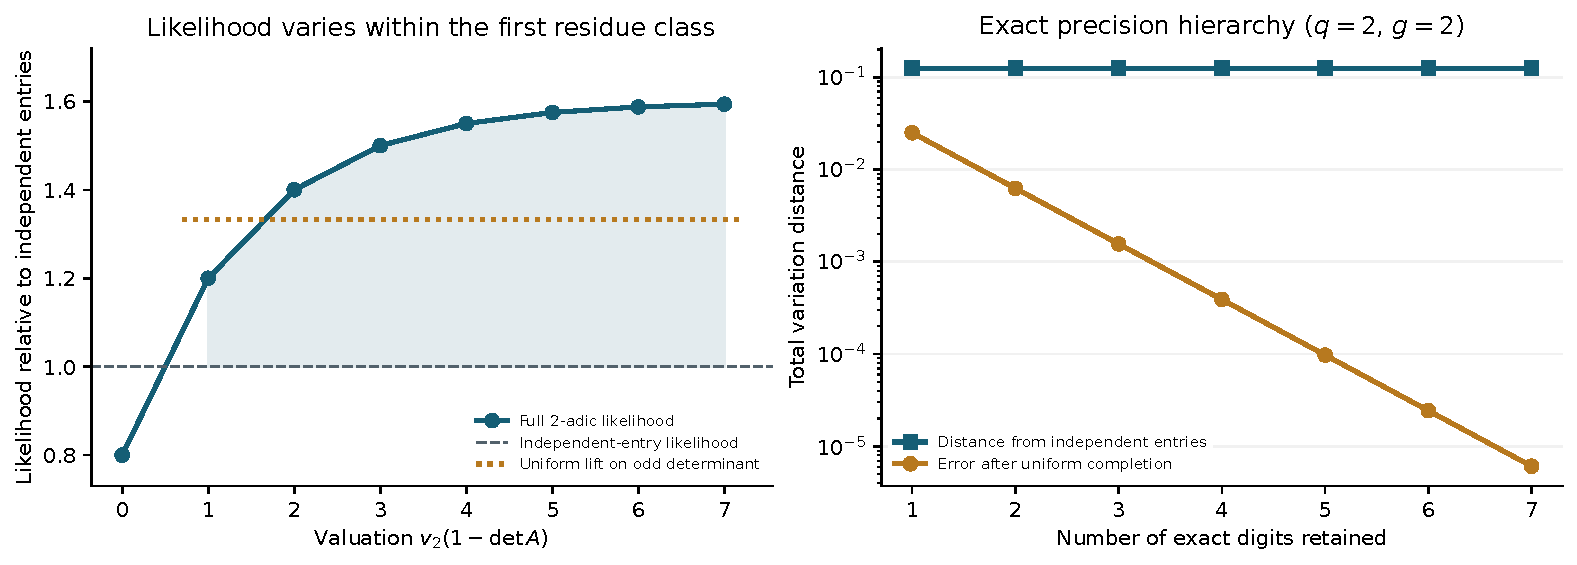
\includegraphics[width=\textwidth]{figures/precision_laws.pdf}
\caption{Left: the complete-ring likelihood for $q=2,g=2$ changes with
the determinant-defect valuation but remains above one for every positive
valuation. Right: the exact uniform-completion error decreases with retained
precision, while the distance from independent entries stays fixed.
All plotted values are evaluations of proved formulas.}
\label{fig:precision}
\end{figure}

\subsection{The complete optimal-threshold curve}

The exact density also describes tests with unequal costs or unequal
prior probabilities. Put $E_r=\{A:1-\det A\in\pi^r\OO\}$ for $r\ge1$
and $\beta_q=(q^2-1)/q^3$. Under the two complete-ring laws,
\begin{align}
 \nu_\infty(E_r)&=\beta_q q^{-(r-1)},\label{eq:roc-uniform}\\
 \mu_\infty(E_r)&=\beta_q q^{-(r-1)}
 \frac{(1-q^{-N})\sum_{j=0}^{r-1}q^{-(N-1)j}
       +q^{-(N-1)r}}{1-q^{-2g}}.\label{eq:roc-symplectic}
\end{align}
Indeed, the first formula follows by varying a unit pivot, and the
second is the finite-$r$ likelihood on the zero-defect class multiplied
by its uniform probability. Because the complete-ring likelihood is
strictly increasing with the valuation, likelihood-threshold tests
are exactly these congruence events, together with the empty or full
event and possible randomization on a level set.

For $q=2,g=2$, the first three threshold points
$(\nu(E_r),\mu(E_r))$ are
\[
 \left(\frac38,\frac12\right),\qquad
 \left(\frac3{16},\frac{11}{40}\right),\qquad
 \left(\frac3{32},\frac{23}{160}\right).
\]
Their largest vertical difference is the first, namely $1/8$.
Different likelihood thresholds can favor the later points; the
one-digit result is therefore not a claim of statistical sufficiency
for every decision problem.

\subsection{Cokernels and dimensions}

In the same binary example a Haar independent matrix has trivial
cokernel with probability $3/8$. The symplectic corner has trivial
cokernel with probability $1/2$. Every nontrivial type has probability
$4/5$ of its independent-model probability. For example,
\[
 \Pr\bigl(\coker M\simeq\mathbb Z_2/(2)\bigr)=\frac9{40},\qquad
 \Pr\bigl(\coker M\simeq(\mathbb Z_2/(2))^2\bigr)=\frac3{160}.
\]
After conditioning on nontrivial cokernel, the factor cancels and the
two entire module distributions agree exactly.

\begin{center}
\begin{tabular}{@{}cccc@{}}
\toprule
$q$ & $g$ & $\TV(\mu_e,\nu_e)$, all $e$ & $\TV(\mu_e,\widetilde\mu_{1,e})$, $e\ge2$\\
\midrule
$2$ & $2$ & $1/8$ & $1/40$\\
$2$ & $3$ & $5/168$ & $1/672$\\
$3$ & $2$ & $19/270$ & $1/135$\\
$3$ & $3$ & $19/2457$ & $2/22113$\\
\bottomrule
\end{tabular}
\end{center}
The exact distances depend on the residue cardinality, the symplectic
dimensions, and the precision in the specified way. They do not
depend on a ramification index or on whether the fraction field has
characteristic zero. This follows from the proofs and is corroborated
by the different finite-ring models tested below.

\section{Verification, reproduction, and limits}
\label{sec:verification}

\subsection{What the computations verify}

The main validation script does not sample random matrices. It
exhaustively enumerates ordered vector pairs $(v,w)$ with symplectic
pairing one, records every projected corner, and compares every
output probability with the exact rational density. Transitivity
proved above identifies this uniform frame experiment with the
appropriate Haar-group compression. Direct integer counts are
independent of the valuation formula being tested.

Across twelve ring-and-dimension cases, the script examined
\textbf{110,894,547 ordered pairs}, found
\textbf{14,979,168 symplectic frames}, and compared
\textbf{20,067 output-matrix probabilities}. All comparisons passed.
The cases include $\mathbb Z/2$, $\mathbb Z/4$, $\mathbb Z/8$,
$\mathbb Z/3$, $\mathbb Z/9$, $\mathbb F_4$,
$\mathbb F_2[t]/(t^2)$, $\mathbb F_2[t]/(t^3)$, and
$\mathbb Z_2[\sqrt2]/((\sqrt2)^3)$, with ambient dimensions four
and six. Together these cases test equal characteristic with
nilpotents, a nonprime residue field, and ramification.

The same script checks normalization, likelihood signs, both exact
distance formulas, the full lower-precision hierarchy, and the
$8/5$ rejection envelope for 704 parameter triples, using rational
arithmetic. It also enumerates all 67 subspaces of $\mathbb F_2^4$
and all 4,489 ordered pairs of these subspaces, verifying the
differential rank $ab-\binom{s}{2}$ for each pair.
These finite checks corroborate the proofs; they are not substitutes
for the proofs or a formal proof-assistant certification.

The taller-corner extension was checked separately over $\mathbb F_2$
in ambient dimensions six and eight, and over $\mathbb F_3$ in dimension
six, always with four visible coordinates. All 7,073 output probabilities
agreed with Corollary~\ref{cor:taller}. These additional checks are not
included in the twelve-case totals above.

An independent implementation separately enumerated all frames
over $\mathbb Z/4$, $\mathbb F_2[t]/(t^2)$ and $\mathbb F_4$, and
again matched every likelihood. The accompanying review checked
the mathematical arguments, with special attention to the terminal
finite-ring term, the characteristic-two lifting step, and the
distinction between the two total-variation comparisons. This is
an independent computational and derivational check within this
research workflow, not external peer review.

\subsection{Reproducible contents}

\begin{center}
\small
\begin{tabularx}{\textwidth}{@{}p{0.37\textwidth}>{\raggedright\arraybackslash}X@{}}
\toprule
Artifact & Purpose \\
\midrule
\artifact{report.tex}, \artifact{sections/} & Complete LaTeX source and
all mathematical arguments. \\
\artifact{report.pdf} & Compiled paper. \\
\artifact{code/verify.py} & Exhaustive finite-ring and tangent-rank
checks; writes \artifact{results/verification.json}. \\
\artifact{code/independent_ring_check.py} & Separate small-ring
implementation using ordinary Python loops and rational numbers. \\
\artifact{code/sample.py} & Exact rational rejection sampler for
corners over $\mathbb Z/p^e\mathbb Z$. \\
\artifact{code/figures.py} & Recreates the paper's figure from the
proved formulas. \\
\artifact{provenance/} & Pinned source identities, literature comparison,
and review scope. \\
\artifact{SHA256SUMS} & File-level integrity checks for the package. \\
\bottomrule
\end{tabularx}
\end{center}

Run \artifact{python3 code/verify.py} from the package directory.
NumPy is used only to accelerate exhaustive enumeration; the
arithmetic conclusions are exact integers and rational numbers.
The independent checker and the sampler use the Python standard
library. For example,
\artifact{python3 code/sample.py --p 2 --g 2 --e 20 --count 5}
samples modulo $2^{20}$ without constructing a full symplectic matrix.
The sampler's ideal-randomness law is exact; the provided command-line
demonstration uses Python's pseudorandom generator.

Recreate the figure with \artifact{python3 code/figures.py}, which
requires Matplotlib and NumPy. Rebuild the paper with
\artifact{latexmk -pdf report.tex}. No new Lean or Rocq theorem is
claimed, and no upstream build output is included as though it were
produced in this investigation.

\subsection{What remains open}

The general rectangular lifting theorem is an exact local criterion,
but not an exact distribution for every choice of large frames.
When both sides contain several symplectic pairs, the residual
alternating Gram matrix is a matrix rather than a scalar. Computing
the resulting complete local density and identifying all frame types
for which first-digit total variation is preserved are natural next
questions. The endpoint $g=1$ already shows that precision preservation
is not automatic.

The $O(q^{-4g})$ assertion holds with fixed residue field and fixed
frame dimensions. When those dimensions grow with $g$, the explicit
two-plane bound in \eqref{eq:padic-B}, rather than the fixed-frame
abbreviation, is the applicable statement. Its sharpness concerns
the distance from a uniform lift of the finite-field law; in the
symplectic-plane example the increase of distance from independent
entries is exactly zero.

Finally, these results furnish local matrix laws that can be used
in arithmetic counting and spanning arguments. They do not by
themselves supply a new global lattice comparison or prove GRH for
any larger class of $L$-functions. Their contribution is a complete,
quantitative passage from finite-field compression to all local
precisions, with exact consequences in the symplectic-pair case.

\bibliographystyle{plain}
\bibliography{references}
\end{document}
